\documentclass[conference]{IEEEtran}
\usepackage{cite}
\usepackage{amsmath,amssymb,amsfonts}
\usepackage{graphicx}
\usepackage{textcomp}
\usepackage{xcolor}
\usepackage{booktabs}
\usepackage{multirow}
\usepackage{url}
\usepackage{tikz}
\usetikzlibrary{arrows.meta, positioning, shapes.geometric, shadings}

\begin{document}

\title{A Review of Signcryption: Theoretical Advances, Standardization, and the Gap to Practical Deployment}

\author{\IEEEauthorblockN{BAHATI Justin (202540272)}
\IEEEauthorblockA{MSE Information and Network Security}}

\maketitle

\begin{abstract}
Signcryption is a public-key cryptographic primitive that simultaneously provides message confidentiality and authentication in a single logical step, at a cost significantly lower than the traditional ``signature-then-encryption'' approach. Since its introduction by Zheng in 1997, signcryption has accumulated formal security models, constructions under diverse hardness assumptions, extensions to identity-based and elliptic curve settings, and international standardization through ISO/IEC 29150. This paper reviews the signcryption literature, tracing its evolution from Zheng's original ElGamal-based construction through formal security proofs by Baek et al.\ and An et al., to identity-based variants by Malone-Lee and Boyen. A comparative analysis evaluates these schemes across dimensions of efficiency, security guarantees, and underlying mathematical assumptions. Critically, we identify and examine a persistent gap between signcryption's theoretical maturity and its practical deployment: despite proven efficiency advantages and ISO standardization, no major cryptographic library or widely deployed protocol has adopted it. We analyze the contributing factors---ecosystem inertia, modularity concerns, competition from AEAD and hardware-accelerated alternatives, security-model complexity, and post-quantum uncertainty---and identify open challenges and initial steps toward bridging theory to practice.
\end{abstract}

\begin{IEEEkeywords}
Signcryption, digital signature, public-key encryption, identity-based cryptography, ISO/IEC 29150, authenticated encryption.
\end{IEEEkeywords}

\section{Introduction}

Secure and authenticated message delivery is a fundamental requirement in modern communications. Three core security goals must be satisfied simultaneously: \textit{confidentiality}, ensuring that only the intended recipient can read the message; \textit{authenticity}, guaranteeing the identity of the sender and the integrity of the message content; and \textit{non-repudiation}, preventing the sender from later denying having sent the message. In public-key cryptography, these goals have traditionally been addressed by separate primitives: encryption schemes for confidentiality and digital signature schemes for authenticity~\cite{zheng1997}.

The conventional approach to achieving both goals is \textit{signature-then-encryption} (StE), where the sender first signs the message using a digital signature algorithm and then encrypts both the message and the signature using the recipient's public key. While functionally correct, this two-step approach incurs the combined computational and communication cost of both operations independently. As Zheng demonstrated~\cite{zheng1997}, for typical security parameters with 1536-bit moduli, the computational cost of StE based on Schnorr signatures and ElGamal encryption requires six modular exponentiations and produces a communication overhead exceeding half the message length.

In 1997, Zheng introduced \textit{signcryption}, a cryptographic primitive that fulfills both functions of digital signature and public-key encryption simultaneously, but with a cost \textit{significantly smaller} than that required by StE~\cite{zheng1997}. The original construction achieved savings of approximately 50\% in computational cost and 85\% in communication overhead compared to StE approaches based on the discrete logarithm problem.

Since this seminal work, signcryption has attracted significant research attention. Formal security models have been established~\cite{baek2002, an2002, baek2007}, the primitive has been extended to elliptic curve settings~\cite{zheng1998} and identity-based frameworks~\cite{malonelee2002, boyen2003}, and alternative constructions based on integer factorization have been proposed~\cite{steinfeld2000}. The culmination of this theoretical development was the publication of ISO/IEC 29150 in 2011~\cite{iso29150}, establishing signcryption as an internationally standardized cryptographic mechanism.

Yet despite this theoretical richness and formal standardization, a striking gap persists: signcryption has seen virtually no adoption in major deployed cryptographic protocols or libraries. TLS 1.3, Signal, S/MIME, and PGP all continue to use separate signature and encryption operations or authenticated encryption with associated data (AEAD) constructions.

The objectives of this review are threefold: (1) to trace the evolution of signcryption from its original proposal through its various extensions, (2) to comparatively analyze the security models and efficiency of existing schemes, and (3) to critically examine why practical deployment has not followed theoretical maturity, identifying what is needed to bridge this gap. We argue that signcryption's deployment failure is fundamentally a \textit{security model communication failure}: the field never produced a simple, practitioner-facing answer to what signcryption offers that the established combination of ECDH and ECDSA does not, and the recent constructive resolution by Badertscher et al.~\cite{badertscher2018}---which proves insider security is the canonical notion---represents the first credible candidate for that answer.

\section{Literature Review}

\subsection{Constructions and Efficiency}

Zheng~\cite{zheng1997} introduced signcryption by observing that no one had previously questioned whether the cost of secure and authenticated message delivery must equal the sum of the costs of signature and encryption separately. He defined a signcryption scheme as a pair of algorithms $(S, U)$ satisfying three properties: \textit{unique unsigncryptability} (the original message can be unambiguously recovered), \textit{security} (the scheme simultaneously provides confidentiality, unforgeability, and non-repudiation), and \textit{efficiency} (the computational and communication cost is strictly less than StE).

Fig.~\ref{fig:ste_vs_sc} illustrates the fundamental difference between the two approaches. In the StE paradigm, the sender performs two independent cryptographic operations sequentially, each consuming separate computational resources and contributing independently to the communication overhead. Signcryption, by contrast, combines these operations into a single cryptographic step that shares internal computations.

\begin{figure}[t]
\centering
\resizebox{\columnwidth}{!}{%
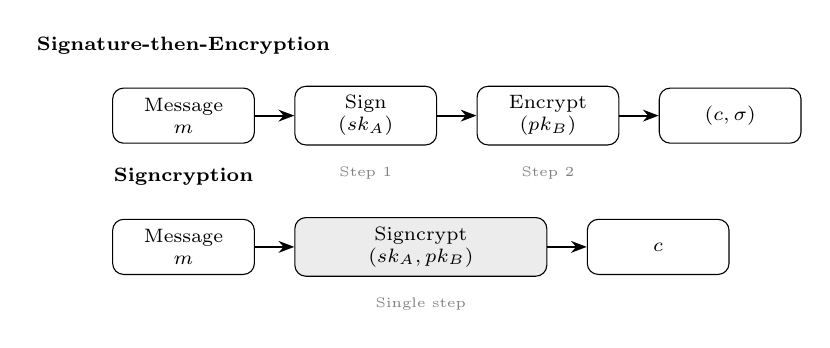
\begin{tikzpicture}[
    node distance=0.6cm and 0.8cm,
    box/.style={draw, rounded corners, minimum width=1.8cm, minimum height=0.7cm, font=\scriptsize, align=center},
    arrow/.style={-{Stealth[length=2mm]}, thick},
    label/.style={font=\scriptsize\bfseries}
]
% StE side
\node[label] (stelabel) {Signature-then-Encryption};
\node[box, below=0.3cm of stelabel] (msg1) {Message\\$m$};
\node[box, right=0.5cm of msg1] (sign) {Sign\\($sk_A$)};
\node[box, right=0.5cm of sign] (enc) {Encrypt\\($pk_B$)};
\node[box, right=0.5cm of enc] (out1) {$(c, \sigma)$};
\draw[arrow] (msg1) -- (sign);
\draw[arrow] (sign) -- (enc);
\draw[arrow] (enc) -- (out1);

% Cost label
\node[below=0.15cm of sign, font=\tiny, text=gray] {Step 1};
\node[below=0.15cm of enc, font=\tiny, text=gray] {Step 2};

% Signcryption side
\node[label, below=1.2cm of stelabel] (sclabel) {Signcryption};
\node[box, below=0.3cm of sclabel] (msg2) {Message\\$m$};
\node[box, right=0.5cm of msg2, minimum width=3.2cm, fill=gray!15] (sc) {Signcrypt\\($sk_A, pk_B$)};
\node[box, right=0.5cm of sc] (out2) {$c$};
\draw[arrow] (msg2) -- (sc);
\draw[arrow] (sc) -- (out2);

% Cost label
\node[below=0.15cm of sc, font=\tiny, text=gray] {Single step};

\end{tikzpicture}%
}
\caption{Comparison of the traditional signature-then-encryption (StE) approach with signcryption. StE requires two sequential cryptographic operations, while signcryption achieves both in a single step with shared computations.}
\label{fig:ste_vs_sc}
\end{figure}

The concrete construction was based on shortened ElGamal signature schemes. By exploiting a common algebraic structure between ElGamal-based signatures and ElGamal encryption, Zheng showed that the key exchange component inherent in signing could be reused for encryption, eliminating redundant exponentiations. For 1536-bit moduli, the scheme requires only three modular exponentiations for signcryption and one for unsigncryption, compared to six for StE. The communication overhead was reduced by approximately 85\%, as the signcrypted text avoids the separate signature appendix.

Fig.~\ref{fig:zheng_alg} presents Zheng's original construction at the algorithmic level, making explicit the mechanism by which a single ephemeral value is reused to derive the symmetric key and bind the signature.

\begin{figure}[t]
\centering
\fbox{\parbox{0.92\columnwidth}{\small
\textbf{Zheng's original signcryption (SDSS1)~\cite{zheng1997}.} Public parameters: primes $p, q$ with $q \mid p-1$; generator $g \in \mathbb{Z}_p^{*}$ of order $q$; one-way hash $H$; keyed hash $\mathrm{KH}$; symmetric cipher $(E, D)$. Alice's key pair: $(x_A,\, y_A{=}g^{x_A})$; Bob's: $(x_B,\, y_B{=}g^{x_B})$.
\vspace{0.35em}

\textbf{Signcrypt}$(m;\, x_A,\, y_B)$:\\
\hspace*{1em}1.\ Pick $x \xleftarrow{\$} \mathbb{Z}_q$;\ \ $(k_1, k_2) \gets H(y_B^{\,x} \bmod p)$\\
\hspace*{1em}2.\ $c \gets E_{k_1}(m)$;\ \ $r \gets \mathrm{KH}_{k_2}(m)$;\ \ $s \gets x / (r + x_A) \bmod q$\\
\hspace*{1em}3.\ Return $(c, r, s)$
\vspace{0.25em}

\textbf{Unsigncrypt}$((c, r, s);\, y_A,\, x_B)$:\\
\hspace*{1em}1.\ $(k_1, k_2) \gets H\bigl((y_A \cdot g^{\,r})^{\,s \cdot x_B} \bmod p\bigr)$\\
\hspace*{1em}2.\ $m \gets D_{k_1}(c)$;\ accept iff $r = \mathrm{KH}_{k_2}(m)$
}}
\caption{The ephemeral value $y_B^{\,x}$ simultaneously (i) derives the symmetric key that encrypts $m$ and (ii) binds the signature component $(r, s)$ via Bob's public key. This sharing---impossible when signing and encrypting are performed as independent primitives---is the structural source of signcryption's efficiency gains over StE.}
\label{fig:zheng_alg}
\end{figure}

Zheng and Imai~\cite{zheng1998} subsequently extended signcryption to elliptic curve groups, motivated by the increasing importance of elliptic curve cryptography for resource-constrained devices such as smart cards. The elliptic curve signcryption scheme preserves the structural advantages of the original construction while benefiting from the shorter key sizes afforded by the elliptic curve discrete logarithm problem (ECDLP). Their analysis demonstrated a 58\% saving in computational cost and a 40\% reduction in communication overhead compared to signature-then-encryption on elliptic curves. The authors also identified several practical applications, including secure key establishment, secure multicasting, authenticated key recovery, and lightweight electronic transaction protocols.

Zheng's original signcryption and the elliptic curve variant both relied on the discrete logarithm problem. Zheng himself posed the open problem of constructing a signcryption scheme based on the integer factorization problem, which would be computationally independent of DLP. Steinfeld and Zheng~\cite{steinfeld2000} proposed a partial solution by modifying an efficient signature scheme based on the Composite Discrete Logarithm Problem (CDLP), constructing a signcryption scheme whose security relies on the hardness of factoring an RSA modulus $N = pq$. Specifically, they proved existential unforgeability in the random oracle model under the assumption that factoring $N$, given additional parameters $(g, S)$ where $g$ is an element of $\mathbb{Z}_N^*$ of large order, is intractable. The confidentiality of the scheme is based on the Diffie--Hellman problem in $\mathbb{Z}_N^*$. While characterized as a ``partial'' solution---because the security reduction relies on a non-standard variant of the factorization assumption---this work demonstrated that signcryption is not inherently tied to DLP-based constructions and opened a path toward diversifying the mathematical foundations of signcryption.

\subsection{Security Models and Proofs}

A critical limitation of Zheng's original work was the absence of formal, reductionist security proofs. While the scheme was argued to be secure based on the intractability of the discrete logarithm problem, no rigorous reduction from a well-defined computational assumption was provided. The motivation for formal proofs was in part catalyzed by Petersen and Michels~\cite{petersen1998}, who identified that Zheng's non-repudiation mechanism inadvertently created a tension with confidentiality, exposing a subtle design trade-off that informal arguments had missed. This gap was addressed by two independent and complementary works in 2002.

Baek, Steinfeld, and Zheng~\cite{baek2002} proposed the first precise security model specifically designed for signcryption schemes. They defined confidentiality through indistinguishability under adaptive chosen ciphertext attack in a model they termed FSO/FUO-IND-CCA2, where the attacker has access to both signcryption and unsigncryption oracles. For unforgeability, they defined existential unforgeability under adaptive chosen message attack (FSO-UF-CMA). A key contribution was demonstrating that Zheng's original scheme is provably secure in the random oracle model: its confidentiality reduces to the Gap Diffie--Hellman (GDH) problem, while its unforgeability reduces to the discrete logarithm problem. An important observation from this work is that the simple ``Encrypt-then-Sign'' (EtS) composition is \textit{completely insecure} against adaptive chosen ciphertext attack in the asymmetric setting, even when the underlying encryption scheme is CCA2-secure. This is because an adversary can strip the sender's signature, replace it with their own, and present a valid ciphertext to the recipient. Fig.~\ref{fig:ets_attack} illustrates this attack. This finding underscores that signcryption is not merely an optimization of StE but provides qualitatively different security properties.

\begin{figure}[t]
\centering
\resizebox{\columnwidth}{!}{%
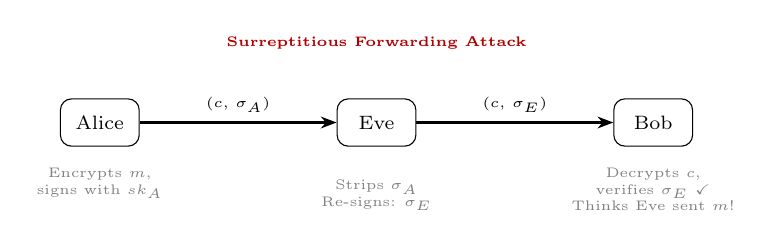
\begin{tikzpicture}[
    node distance=0.4cm,
    entity/.style={draw, rounded corners, minimum width=1cm, minimum height=0.6cm, font=\scriptsize, align=center, fill=white},
    arrow/.style={-{Stealth[length=2mm]}, thick},
    note/.style={font=\tiny, text=gray, align=center}
]
% Entities
\node[entity] (alice) {Alice};
\node[entity, right=2.5cm of alice] (eve) {Eve};
\node[entity, right=2.5cm of eve] (bob) {Bob};

% Step 1: Alice sends
\draw[arrow] (alice) -- node[above, font=\tiny] {$(c,\, \sigma_A)$} (eve);
\node[note, below=0.15cm of alice] {Encrypts $m$,\\signs with $sk_A$};

% Step 2: Eve re-signs
\node[note, below=0.3cm of eve] {Strips $\sigma_A$\\Re-signs: $\sigma_E$};

% Step 3: Eve forwards
\draw[arrow] (eve) -- node[above, font=\tiny] {$(c,\, \sigma_E)$} (bob);
\node[note, below=0.15cm of bob] {Decrypts $c$,\\verifies $\sigma_E$ \checkmark\\Thinks Eve sent $m$!};

% Attack label
\node[font=\tiny\bfseries, text=red!70!black, above=0.5cm of eve] {Surreptitious Forwarding Attack};

\end{tikzpicture}%
}
\caption{The Encrypt-then-Sign (EtS) attack in the asymmetric setting. Eve intercepts Alice's ciphertext, strips $\sigma_A$, re-signs with her own key, and forwards to Bob who believes Eve authored the message.}
\label{fig:ets_attack}
\end{figure}

The extended journal version~\cite{baek2007} further refined these models with flexible signcryption/unsigncryption oracles that allow the attacker to choose both messages and public keys when querying oracles.

More recently, Badertscher, Banfi, and Maurer~\cite{badertscher2018} provided a constructive perspective on signcryption security that resolves much of the confusion surrounding competing security models. Working within the constructive cryptography framework, they proved from first principles that \textit{insider security}---where the adversary may be a legitimate user of the system---is the canonical security notion for signcryption. This result is significant because it demonstrates that the seemingly complex landscape of two-user versus multi-user models and insider versus outsider adversaries reduces to a single, well-motivated definition. Their analysis places signcryption on a firm foundational footing that had been lacking despite the proliferation of security models.

Independently, An, Dodis, and Rabin~\cite{an2002} studied the security of joint signature and encryption from a compositional perspective. They presented two security definitions depending on whether the adversary is an outsider or an insider (a legal user of the system). They examined three generic sequential composition methods---``Encrypt-then-Sign'' ($\mathcal{E}t\mathcal{S}$), ``Sign-then-Encrypt'' ($\mathcal{S}t\mathcal{E}$), and a novel ``Commit-then-Encrypt-and-Sign'' ($\mathcal{C}t\mathcal{E}\&\mathcal{S}$)---and showed that, contrary to negative results in the symmetric setting, both $\mathcal{E}t\mathcal{S}$ and $\mathcal{S}t\mathcal{E}$ are secure in the public-key setting under appropriate definitions. The $\mathcal{C}t\mathcal{E}\&\mathcal{S}$ method is notable for applying signature and encryption operations \textit{in parallel}, potentially offering efficiency gains over sequential approaches. They also proposed generalized CCA2-security (gCCA2), a slight relaxation of standard CCA2 that resolves definitional shortcomings while sufficing for all known applications.

\subsection{Identity-Based and Certificateless Settings}

Identity-based (IB) cryptography, originally proposed by Shamir in 1984 and made practical by Boneh and Franklin's identity-based encryption (IBE) scheme in 2001~\cite{boneh2001}, allows any arbitrary string (such as an email address) to serve as a public key, eliminating the need for certificate-based public key infrastructure. Extending signcryption to the identity-based setting is a natural and practically motivated goal.

Malone-Lee~\cite{malonelee2002} proposed the first identity-based signcryption scheme using bilinear pairings on elliptic curves. The scheme consists of four algorithms---Setup, Extract, Signcrypt, and Unsigncrypt---and operates under the Bilinear Diffie--Hellman (BDH) assumption. Malone-Lee defined two security notions tailored to the IB setting: \textit{indistinguishability of identity-based signcryptions under chosen ciphertext attack} (IND-ISC-CCA) for confidentiality, and \textit{existential unforgeability of identity-based signcryptions under adaptive chosen message attack} (EF-ISC-ACMA) for unforgeability. The scheme provides non-repudiation through a verification equation that a third party can check independently. An efficiency comparison showed that the signcryption approach requires fewer pairing computations than a naive composition of separate IBE and IB signature schemes. However, subsequent cryptanalysis by Libert and Quisquater~\cite{libert2003} revealed that Malone-Lee's construction inadvertently exposed the digital signature in the clear within the signcryptext structure, allowing an adversary who could guess the plaintext to verify their guess via the exposed signature without breaking the encryption layer, thereby defeating semantic security. Libert and Quisquater proposed corrected schemes that fully masked the signature components within the symmetric encryption layer, and provided rigorous proofs under the Decisional Bilinear Diffie--Hellman (DBDH) assumption. This episode illustrates a recurring pattern in signcryption research: achieving the correct integration of signature and encryption components is subtle, and seemingly secure constructions can harbor vulnerabilities that only surface under careful formal analysis.

Boyen~\cite{boyen2003} proposed a more ambitious identity-based signature/encryption (IBSE) scheme that satisfies a broader set of security requirements beyond basic confidentiality and unforgeability. In addition to IND-CCA2 confidentiality and existential unforgeability against chosen-message insider attacks, Boyen's scheme provides: \textit{ciphertext anonymity} (hiding sender and recipient identities from outsiders), \textit{ciphertext unlinkability} (allowing the sender to disavow creating a ciphertext for any given recipient), and \textit{ciphertext authentication} (allowing only the legitimate recipient to verify that the ciphertext was crafted by the claimed sender). The construction uses a two-layer ``sign-then-encrypt'' design with a detachable randomized signature followed by anonymous deterministic encryption. This architecture is more modular and secure than ``monolithic'' signcryption designs that combine signing and encryption into a single inseparable operation. Furthermore, the scheme naturally supports multi-recipient encryption with signature sharing, offering scalability advantages. Notably, Boyen's use of ephemeral randomization provides \textit{forward secrecy}---the property that compromise of long-term keys does not expose past communications---a security guarantee absent from Zheng's original construction and increasingly demanded by modern protocol designers.

Fig.~\ref{fig:key_mgmt} contrasts the key management architectures across the three paradigms relevant to signcryption: traditional PKI, identity-based cryptography, and the certificateless approach---introduced by Barbosa and Farshim~\cite{barbosa2008} and discussed further in Section~IV---that resolves the key escrow problem.

\begin{figure}[t]
\centering
\resizebox{\columnwidth}{!}{%
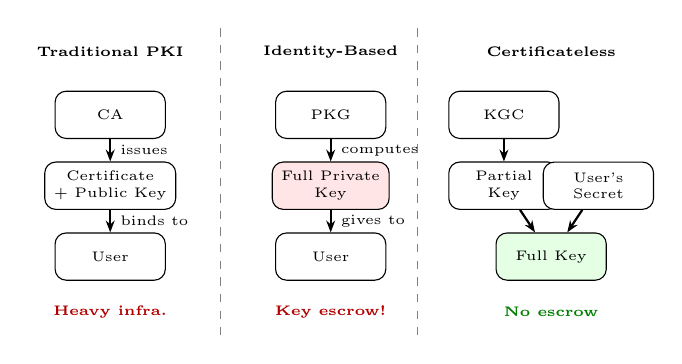
\begin{tikzpicture}[
    box/.style={draw, rounded corners, minimum width=1.4cm, minimum height=0.6cm, font=\tiny, align=center, fill=white},
    arrow/.style={-{Stealth[length=1.5mm]}, thick},
    title/.style={font=\tiny\bfseries, align=center},
    warn/.style={font=\tiny\bfseries, text=red!70!black},
    ok/.style={font=\tiny\bfseries, text=green!50!black},
    sep/.style={draw=gray, dashed}
]

% --- PKI Column ---
\node[title] (t1) at (0, 2.8) {Traditional PKI};
\node[box] (ca) at (0, 2) {CA};
\node[box] (cert) at (0, 1.1) {Certificate\\+ Public Key};
\node[box] (user1) at (0, 0.2) {User};
\draw[arrow] (ca) -- node[right, font=\tiny] {issues} (cert);
\draw[arrow] (cert) -- node[right, font=\tiny] {binds to} (user1);
\node[warn] at (0, -0.5) {Heavy infra.};

% --- IBC Column ---
\node[title] (t2) at (2.8, 2.8) {Identity-Based};
\node[box] (pkg) at (2.8, 2) {PKG};
\node[box, fill=red!10] (fullkey) at (2.8, 1.1) {Full Private\\Key};
\node[box] (user2) at (2.8, 0.2) {User};
\draw[arrow] (pkg) -- node[right, font=\tiny] {computes} (fullkey);
\draw[arrow] (fullkey) -- node[right, font=\tiny] {gives to} (user2);
\node[warn] at (2.8, -0.5) {Key escrow!};

% --- CLC Column ---
\node[title] (t3) at (5.6, 2.8) {Certificateless};
\node[box] (kgc) at (5, 2) {KGC};
\node[box] (partial) at (5, 1.1) {Partial\\Key};
\node[box] (secret) at (6.2, 1.1) {User's\\Secret};
\node[box, fill=green!10] (full2) at (5.6, 0.2) {Full Key};
\draw[arrow] (kgc) -- (partial);
\draw[arrow] (partial) -- (full2);
\draw[arrow] (secret) -- (full2);
\node[ok] at (5.6, -0.5) {No escrow};

% Separators
\draw[sep] (1.4, 3.1) -- (1.4, -0.8);
\draw[sep] (3.9, 3.1) -- (3.9, -0.8);

\end{tikzpicture}%
}
\caption{Evolution of key management paradigms. PKI requires certificate infrastructure. Identity-based cryptography eliminates certificates but introduces key escrow. Certificateless cryptography resolves both by splitting key generation between KGC and user.}
\label{fig:key_mgmt}
\end{figure}

\subsection{Standardization: ISO/IEC 29150}

The theoretical development of signcryption reached a significant milestone with the publication of ISO/IEC 29150:2011, titled ``Information technology -- Security techniques -- Signcryption''~\cite{iso29150}. This international standard specifies signcryption mechanisms based on the discrete logarithm problem, including variants on elliptic curves, drawing directly from the constructions and security analyses developed by Zheng and subsequent researchers.

The standard defines two families of signcryption mechanisms. The first family is based on the discrete logarithm problem in finite fields, directly descended from Zheng's original SDSS1 and SDSS2 (Shortened Digital Signature Standard) constructions~\cite{zheng1997}. The second family operates on elliptic curve groups, building on the work of Zheng and Imai~\cite{zheng1998}. For each family, the standard specifies both \textit{key transport} signcryption---where a fresh symmetric key is generated and transmitted alongside the encrypted message---and \textit{key agreement} signcryption---where the symmetric key is derived from a shared Diffie--Hellman computation. The standard provides concrete parameter recommendations, including minimum key sizes, approved hash functions, and symmetric encryption algorithms to be used within the signcryption framework.

The existence of an ISO standard represents formal recognition by the international standards community that signcryption is a well-defined, secure, and useful cryptographic primitive. However, standardization has not translated into adoption. Unlike AES or SHA-3, which were driven by NIST competitions with broad industry participation, ISO/IEC 29150 was developed without a corresponding push for reference implementations or industry champion support. No major cryptographic library has published a conforming implementation, and no widely deployed protocol references the standard. This stands in contrast to other ISO cryptographic standards that have seen broader uptake, and highlights that standardization is a necessary but insufficient condition for practical deployment.

Fig.~\ref{fig:timeline} summarizes the chronological development of signcryption from its inception to standardization, illustrating the progression from efficiency-motivated construction to formally proven and standardized primitive.

\begin{figure*}[t]
\centering
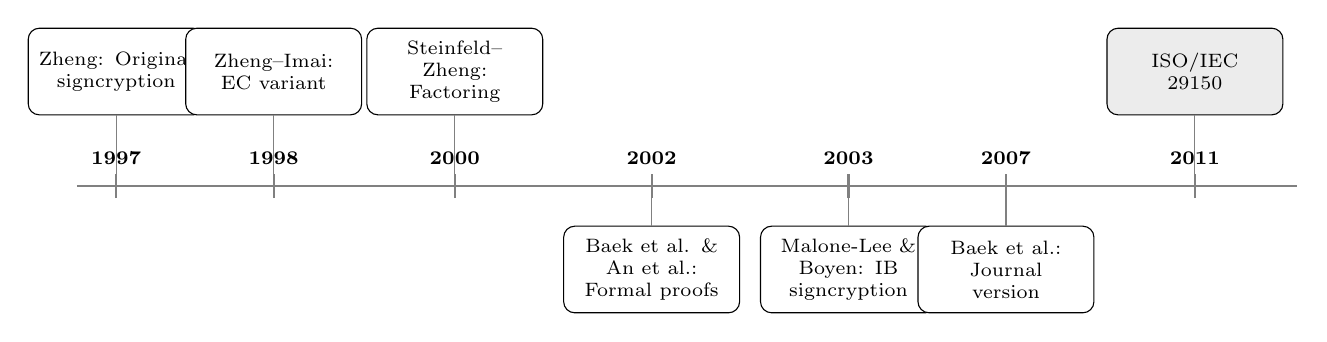
\begin{tikzpicture}[
    event/.style={draw, rounded corners, fill=white, text width=2.0cm, font=\scriptsize, align=center, minimum height=1.1cm},
    arrow/.style={-{Stealth[length=2mm]}, thick, gray},
]
% Timeline line
\draw[thick, gray] (0,0) -- (15.5,0);

% Year markers - all placed above the line
\foreach \x/\year in {0.5/1997, 2.5/1998, 4.8/2000, 7.3/2002, 9.8/2003, 11.8/2007, 14.2/2011} {
    \draw[thick, gray] (\x, -0.15) -- (\x, 0.15);
    \node[above, font=\scriptsize\bfseries] at (\x, 0.15) {\year};
}

% Events above timeline (connected with lines going up)
\node[event, above=0.9cm] (e1) at (0.5, 0) {Zheng: Original signcryption};
\node[event, above=0.9cm] (e2) at (2.5, 0) {Zheng--Imai: EC variant};
\node[event, above=0.9cm] (e3) at (4.8, 0) {Steinfeld--Zheng: Factoring};
\node[event, above=0.9cm, fill=gray!15] (e7) at (14.2, 0) {ISO/IEC\\29150};

% Events below timeline (with enough spacing)
\node[event, below=0.5cm] (e4) at (7.3, 0) {Baek et al. \&\\An et al.:\\Formal proofs};
\node[event, below=0.5cm] (e5) at (9.8, 0) {Malone-Lee \&\\Boyen: IB\\signcryption};
\node[event, below=0.5cm] (e6) at (11.8, 0) {Baek et al.:\\Journal\\version};

% Connecting lines
\draw[gray, thin] (0.5, 0.15) -- (e1);
\draw[gray, thin] (2.5, 0.15) -- (e2);
\draw[gray, thin] (4.8, 0.15) -- (e3);
\draw[gray, thin] (14.2, 0.15) -- (e7);
\draw[gray, thin] (7.3, -0.15) -- (e4);
\draw[gray, thin] (9.8, -0.15) -- (e5);
\draw[gray, thin] (11.8, -0.15) -- (e6);

\end{tikzpicture}
\caption{Timeline of key developments in signcryption research, from Zheng's 1997 original proposal to ISO/IEC 29150 standardization in 2011.}
\label{fig:timeline}
\end{figure*}

\section{Analysis and Discussion}

\subsection{Comparative Analysis of Signcryption Schemes}

Table~\ref{tab:comparison} presents a comparative summary of the signcryption schemes reviewed in this paper across multiple dimensions.

\begin{table*}[t]
\centering
\caption{Comparative Analysis of Signcryption Schemes}
\label{tab:comparison}
\begin{tabular}{@{}lcclllll@{}}
\toprule
\textbf{Scheme} & \textbf{Year} & \textbf{Setting} & \textbf{Hardness} & \textbf{Proof Model} & \textbf{Confidentiality} & \textbf{Unforgeability} & \textbf{Efficiency vs StE} \\
\midrule
Zheng~\cite{zheng1997} & 1997 & PKI & DLP & --- & Informal & Informal & 50\%/85\% savings \\
Zheng--Imai~\cite{zheng1998} & 1998 & PKI (EC) & ECDLP & --- & Informal & Informal & 58\%/40\% savings \\
Steinfeld--Zheng~\cite{steinfeld2000} & 2000 & PKI & Factoring & ROM & --- & ROM proof & Comparable \\
Baek et al.~\cite{baek2002,baek2007} & 2002 & PKI & GDH / DLP & ROM & IND-CCA2 & EUF-CMA & Same as Zheng \\
An et al.~\cite{an2002} & 2002 & PKI & Generic & ROM & gCCA2 & sUF-CMA & Composition-based \\
Malone-Lee~\cite{malonelee2002} & 2002 & ID-based & BDH & ROM & IND-ISC-CCA & EF-ISC-ACMA & Fewer pairings \\
Boyen~\cite{boyen2003} & 2003 & ID-based & BDH & ROM & IND-CCA2 & EUF-CMA & Compact \\
Sato--Shikata~\cite{sato2018} & 2018 & PKI & LWE / SIS & Standard & IND-CCA2 & EUF-CMA & Under study \\
\bottomrule
\end{tabular}
\end{table*}

Several trends emerge from this comparison. First, the field has progressed from informal security arguments to rigorous, reductionist proofs under well-studied computational assumptions. Second, the underlying hardness assumptions have diversified from DLP alone to include integer factorization, the Gap Diffie--Hellman problem, and bilinear Diffie--Hellman assumptions. Third, the operational setting has expanded from traditional PKI to identity-based frameworks, broadening the potential applicability of signcryption. Fourth, the Proof Model column reveals a critical observation: every scheme with formal proofs prior to 2018 relies on the random oracle model (ROM), an idealized assumption that does not hold in practice. Only the lattice-based construction of Sato and Shikata~\cite{sato2018} achieves security in the standard model, meaning that for all widely studied signcryption schemes, real-world security guarantees are weaker than the proofs formally establish. This distinction is directly relevant to deployment confidence.

The efficiency advantages demonstrated by the original schemes---50\% computational savings and up to 85\% communication savings---remain relevant, particularly for constrained environments. The elliptic curve variant~\cite{zheng1998} is especially significant given the widespread adoption of ECC in modern cryptographic practice.

\subsection{The Theory--Practice Gap}

Perhaps the most striking finding of this review is the disconnect between signcryption's theoretical maturity and its deployment in mainstream software. By any academic measure, signcryption is a well-established primitive: it has formal security definitions, provably secure constructions under standard assumptions, multiple variants for different settings, and an international standard (ISO/IEC 29150). Yet no major cryptographic library---not OpenSSL, not libsodium, not BoringSSL---implements signcryption natively. No widely deployed protocol---not TLS, not Signal, not S/MIME---uses it.

It is important to note, however, that signcryption \textit{is} gaining meaningful traction in resource-constrained domains. Recent literature (2024--2025) documents active adoption of certificateless and lightweight signcryption schemes in IoT sensor networks~\cite{iotsigncryption2025}, the Internet of Medical Things (IoMT) for secure health data transmission from wearable devices, and vehicular ad-hoc networks (VANETs) for authenticated vehicle-to-infrastructure communication. In these environments, where computational budgets and communication bandwidth are severely limited, signcryption's efficiency advantages over separate sign-then-encrypt pipelines are not merely theoretical but operationally decisive. Adoption thus follows a clear gradient: the more constrained the environment, the more compelling signcryption becomes. Fig.~\ref{fig:adoption} visualizes this adoption spectrum.

\begin{figure}[!htbp]
\centering
\resizebox{\columnwidth}{!}{%
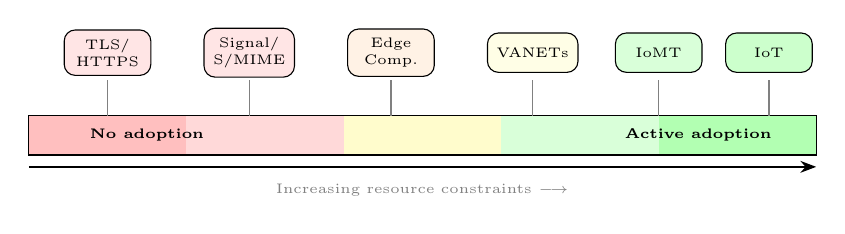
\begin{tikzpicture}[
    dbox/.style={draw, rounded corners, minimum height=0.5cm, minimum width=1.1cm, font=\tiny, align=center, fill=white},
    arrow/.style={-{Stealth[length=2mm]}, thick},
]

% Gradient bar using colored segments
\fill[red!25] (0,0) rectangle (2, 0.5);
\fill[red!15] (2,0) rectangle (4, 0.5);
\fill[yellow!20] (4,0) rectangle (6, 0.5);
\fill[green!15] (6,0) rectangle (8, 0.5);
\fill[green!30] (8,0) rectangle (10, 0.5);
\draw (0,0) rectangle (10, 0.5);

% Labels on gradient
\node[font=\tiny\bfseries] at (1.5, 0.25) {No adoption};
\node[font=\tiny\bfseries] at (8.5, 0.25) {Active adoption};

% Arrow below
\draw[arrow] (0, -0.15) -- (10, -0.15);
\node[font=\tiny, text=gray] at (5, -0.45) {Increasing resource constraints $\longrightarrow$};

% Domains above - evenly spaced
\node[dbox, fill=red!10] at (1.0, 1.3) {TLS/\\HTTPS};
\node[dbox, fill=red!10] at (2.8, 1.3) {Signal/\\S/MIME};
\node[dbox, fill=orange!10] at (4.6, 1.3) {Edge\\Comp.};
\node[dbox, fill=yellow!10] at (6.4, 1.3) {VANETs};
\node[dbox, fill=green!15] at (8.0, 1.3) {IoMT};
\node[dbox, fill=green!20] at (9.4, 1.3) {IoT};

% Lines connecting to bar
\foreach \x in {1.0, 2.8, 4.6, 6.4, 8.0, 9.4} {
    \draw[gray, thin] (\x, 0.5) -- (\x, 0.95);
}

\end{tikzpicture}%
}
\caption{Signcryption adoption gradient. Adoption increases with resource constraints: absent from mainstream protocols with hardware-accelerated alternatives, but actively deployed in IoT, IoMT, and vehicular networks.}
\label{fig:adoption}
\end{figure}

The gap, therefore, is specifically between signcryption and \textit{mainstream} software infrastructure. This section examines why.

\textbf{Ecosystem Inertia.} The existing cryptographic ecosystem is built around separate signature and encryption primitives. Decades of engineering effort have produced optimized implementations, well-tested libraries, and battle-hardened protocol integrations for RSA, ECDSA, AES-GCM, and similar algorithms. Replacing these with signcryption would require coordinated changes across the entire stack, from hardware acceleration to protocol specifications, with no backward compatibility path.

\textbf{Modularity and Algorithm Agility.} Keeping signature and encryption as separate primitives offers significant practical advantages. When a vulnerability is discovered in an encryption algorithm, it can be replaced without affecting the signature scheme, and vice versa. Protocol designers value this modularity---TLS 1.3's cipher suite negotiation, for example, allows independent selection of key exchange, authentication, and symmetric encryption algorithms. A monolithic signcryption scheme would couple these choices, reducing flexibility.

\textbf{Competition from AEAD and Hardware Acceleration.} In the symmetric setting, authenticated encryption with associated data (AEAD) modes such as AES-GCM and ChaCha20-Poly1305 have largely solved the problem of joint confidentiality and integrity. In the asymmetric setting, hybrid encryption (ECDH key agreement followed by AEAD) combined with separate digital signatures provides a well-understood and widely deployed solution that achieves similar goals to signcryption, albeit at higher theoretical cost. Crucially, dedicated hardware instructions---such as Intel/AMD AES-NI, which accelerates AES-GCM to over 1,300~MB/s, and ARM CryptoCell, which provides hardware-accelerated ECDSA and ECDH on embedded processors---have effectively erased signcryption's efficiency advantage on platforms equipped with these accelerators. Signcryption's computational savings remain operationally significant only on constrained microcontrollers that lack such hardware support, which further explains the adoption gradient observed in Section~III-B.

\textbf{Complexity of Security Models.} The security analysis of signcryption involves subtle distinctions---two-user versus multi-user settings, insider versus outsider adversaries, various oracle access models---that, while theoretically important, add complexity that practitioners may find daunting. The finding by Baek et al.~\cite{baek2002} that simple EtS composition is insecure in the asymmetric setting, while important, also highlights the subtlety of getting signcryption security right. Recent work by Badertscher et al.~\cite{badertscher2018} has provided a constructive resolution by proving that insider security is the canonical notion, which may help reduce this conceptual barrier over time.

\textbf{Post-Quantum Uncertainty.} The ongoing transition to post-quantum cryptography creates uncertainty for any new primitive adoption. All existing signcryption schemes are based on number-theoretic assumptions (DLP, factoring, pairings) that are vulnerable to quantum attacks. Until efficient post-quantum signcryption schemes are developed and analyzed, organizations may reasonably hesitate to invest in deploying a primitive that will need to be replaced.

\section{Challenges and Research Gaps}

Based on our analysis, we identify the following challenges and research gaps, ordered by their dependency relationships. The first two are \textit{foundational}---they block progress on everything downstream. The remaining challenges become tractable only once these foundations are in place.

\textbf{1.\ Post-Quantum Signcryption (Foundation).} All classical signcryption schemes rely on number-theoretic assumptions vulnerable to Shor's algorithm, making this the most urgent theoretical challenge. Recent work by Sato and Shikata~\cite{sato2018} has demonstrated the feasibility of lattice-based signcryption proven secure in the standard model (without random oracles), relying on the Learning With Errors (LWE) and Small Integer Solution (SIS) problems. Independently, G\'{e}rard and Merckx~\cite{gerard2018} proposed a lattice-based construction taking a different approach. While these works represent significant theoretical progress, practical post-quantum signcryption schemes with competitive performance remain an active area, particularly in light of the NIST post-quantum standardization effort. Until this challenge is resolved, any deployment investment risks obsolescence during the quantum transition.

\textbf{2.\ Standard-Model Proofs for Classical Schemes (Foundation).} As Table~\ref{tab:comparison} reveals, every classical signcryption scheme with formal proofs relies on the random oracle model---an idealization that does not hold in practice. Standard-model proofs for efficient DLP- and pairing-based constructions would strengthen deployment confidence and are a prerequisite for the kind of security assurance that protocol designers demand. Sato and Shikata's lattice-based scheme is currently the only construction with standard-model proofs, but its performance characteristics differ substantially from the classical schemes that practitioners would most readily adopt.

\textbf{3.\ Library Implementations (Enabler).} The availability of signcryption in mainstream cryptographic libraries is a prerequisite for all downstream adoption. Without reference implementations, protocol designers cannot evaluate signcryption in practice, and IoT developers cannot benchmark against real hardware. A conforming implementation of ISO/IEC 29150~\cite{iso29150} in a widely used library such as libsodium would be a practical first step.

\textbf{4.\ Protocol Integration (Depends on 3).} Concrete proposals for integrating signcryption into existing protocol frameworks---such as TLS, DTLS for IoT, or CoAP---require working library implementations as a starting point. This challenge is not purely algorithmic: it demands protocol engineering, composed-setting security analysis, and backward compatibility strategies with existing cipher suite negotiation mechanisms.

\textbf{5.\ Lightweight Implementations for IoT (Depends on 1, 3).} While recent work has demonstrated signcryption's viability in IoT, IoMT, and vehicular networks, most proposals remain at the theoretical or simulation stage. Production-grade implementations require validated performance on specific microcontroller platforms, integration into IoT protocol stacks such as CoAP and MQTT, and resistance to side-channel attacks on constrained hardware. This challenge depends on both post-quantum foundations (since IoT devices have long deployment lifetimes) and library availability.

\textbf{6.\ Key Escrow in Identity-Based Settings (Parallel).} Identity-based signcryption inherits the key escrow problem from IBE: the trusted authority that generates private keys can decrypt all messages and forge all signatures. Barbosa and Farshim~\cite{barbosa2008} addressed this through \textit{certificateless signcryption}, where the key generation center produces only a partial private key and the user independently generates a secret value to form their full key. While this eliminates key escrow without reintroducing certificates, the dual-adversary security model adds analytical complexity, and pairing-free constructions for constrained devices remain an active area. This challenge can be pursued independently of the others.

\textbf{7.\ Multi-Receiver Scalability (Depends on 1).} While Boyen~\cite{boyen2003} demonstrated multi-recipient support through signature sharing, scalability for broadcast or multicast scenarios---particularly with post-quantum constructions, whose ciphertext and key sizes are substantially larger---remains an open question.

\section{Conclusion}

This review has traced the evolution of signcryption from Zheng's 1997 proposal through two and a half decades of theoretical development, culminating in ISO/IEC 29150 standardization. The progression is remarkable: from an informally argued construction to provably secure schemes under well-defined computational assumptions, from a single algebraic setting to identity-based and elliptic curve variants, and from a research curiosity to an international standard.

The comparative analysis reveals that signcryption offers genuine and quantifiable efficiency advantages over the traditional sign-then-encrypt approach---savings of 50--58\% in computation and 40--85\% in communication overhead, depending on the underlying algebraic setting. The formal security models developed by Baek et al.~\cite{baek2002,baek2007} and An et al.~\cite{an2002} provide strong confidence in the security of well-designed signcryption schemes.

Yet the persistent gap between this theoretical maturity and practical deployment represents both a challenge and an opportunity. The factors we have identified---ecosystem inertia, modularity concerns, AEAD competition, security model complexity, and post-quantum uncertainty---are not fundamental barriers but engineering and adoption challenges. ISO/IEC 29150 provides the standardization foundation; what remains is the development of post-quantum constructions, reference library implementations, and protocol integration proposals that can finally bring signcryption from theory into practice.

\begin{thebibliography}{17}

\bibitem{zheng1997}
Y.~Zheng, ``Digital signcryption or how to achieve cost(signature \& encryption) $\ll$ cost(signature) + cost(encryption),'' in \textit{Advances in Cryptology --- CRYPTO '97} (Lecture Notes in Computer Science, vol.~1294), B.~S.~Kaliski~Jr., Ed.\hspace{1em}Berlin, Germany: Springer, 1997, pp.~165--179.

\bibitem{baek2002}
J.~Baek, R.~Steinfeld, and Y.~Zheng, ``Formal proofs for the security of signcryption,'' in \textit{Public Key Cryptography --- PKC 2002} (Lecture Notes in Computer Science, vol.~2274), D.~Naccache and P.~Paillier, Eds.\hspace{1em}Berlin, Germany: Springer, 2002, pp.~80--98.

\bibitem{an2002}
J.~H.~An, Y.~Dodis, and T.~Rabin, ``On the security of joint signature and encryption,'' in \textit{Advances in Cryptology --- EUROCRYPT 2002} (Lecture Notes in Computer Science, vol.~2332), L.~R.~Knudsen, Ed.\hspace{1em}Berlin, Germany: Springer, 2002, pp.~83--107.

\bibitem{baek2007}
J.~Baek, R.~Steinfeld, and Y.~Zheng, ``Formal proofs for the security of signcryption,'' \textit{Journal of Cryptology}, vol.~20, no.~2, pp.~203--235, 2007.

\bibitem{zheng1998}
Y.~Zheng and H.~Imai, ``How to construct efficient signcryption schemes on elliptic curves,'' \textit{Information Processing Letters}, vol.~68, no.~5, pp.~227--233, 1998.

\bibitem{malonelee2002}
J.~Malone-Lee, ``Identity-based signcryption,'' \textit{Cryptology ePrint Archive}, Report 2002/098, 2002.

\bibitem{boyen2003}
X.~Boyen, ``Multipurpose identity-based signcryption: A Swiss army knife for identity-based cryptography,'' in \textit{Advances in Cryptology --- CRYPTO 2003} (Lecture Notes in Computer Science, vol.~2729), D.~Boneh, Ed.\hspace{1em}Berlin, Germany: Springer, 2003, pp.~383--399.

\bibitem{steinfeld2000}
R.~Steinfeld and Y.~Zheng, ``A signcryption scheme based on integer factorization,'' in \textit{Information Security} (Lecture Notes in Computer Science, vol.~1975), J.~Pieprzyk, E.~Okamoto, and J.~Seberry, Eds.\hspace{1em}Berlin, Germany: Springer, 2000, pp.~308--322.

\bibitem{iso29150}
ISO/IEC 29150:2011, ``Information technology --- Security techniques --- Signcryption,'' International Organization for Standardization, Geneva, Switzerland, 2011.

\bibitem{badertscher2018}
C.~Badertscher, F.~Banfi, and U.~Maurer, ``A constructive perspective on signcryption security,'' in \textit{Security and Cryptography for Networks --- SCN 2018} (Lecture Notes in Computer Science, vol.~11035), D.~Catalano and R.~De~Prisco, Eds.\hspace{1em}Cham, Switzerland: Springer, 2018, pp.~102--120.

\bibitem{petersen1998}
H.~Petersen and M.~Michels, ``Cryptanalysis and improvement of signcryption schemes,'' in \textit{IEE Proceedings --- Computers and Digital Techniques}, vol.~145, no.~2, pp.~149--151, 1998.

\bibitem{boneh2001}
D.~Boneh and M.~Franklin, ``Identity-based encryption from the Weil pairing,'' in \textit{Advances in Cryptology --- CRYPTO 2001} (Lecture Notes in Computer Science, vol.~2139), J.~Kilian, Ed.\hspace{1em}Berlin, Germany: Springer, 2001, pp.~213--229.

\bibitem{libert2003}
B.~Libert and J.-J.~Quisquater, ``New identity based signcryption schemes from pairings,'' in \textit{Proc. IEEE Information Theory Workshop (ITW 2003)}, Paris, France, 2003, pp.~155--158.

\bibitem{barbosa2008}
M.~Barbosa and P.~Farshim, ``Certificateless signcryption,'' in \textit{Proc. ACM Symposium on Information, Computer and Communications Security (ASIACCS 2008)}, Tokyo, Japan, 2008, pp.~369--372.

\bibitem{sato2018}
S.~Sato and J.~Shikata, ``Lattice-based signcryption without random oracles,'' in \textit{Post-Quantum Cryptography (PQCrypto 2018)} (Lecture Notes in Computer Science, vol.~10786), T.~Lange and R.~Steinwandt, Eds.\hspace{1em}Cham, Switzerland: Springer, 2018, pp.~331--351.

\bibitem{iotsigncryption2025}
M.~Rahmani, A.~Nitaj, and M.~Ziane, ``IoT-friendly certificateless signcryption schemes: Introducing a provably secure scheme in ROM,'' \textit{Journal of Information Security and Applications}, vol.~89, article 103981, 2025.

\bibitem{gerard2018}
F.~G\'{e}rard and K.~Merckx, ``Post-quantum signcryption from lattice-based signatures,'' \textit{Cryptology ePrint Archive}, Report 2018/861, 2018.

\end{thebibliography}

\end{document}
